\documentclass[a4paper, 14pt]{extarticle}
\usepackage{./styles/generalPreamble}
\usepackage{./styles/longReportFormat}
\usepackage{./styles/russianLocale}
\usepackage{./styles/nonFancyTOC}
\usepackage{./styles/sourceCode}
\usepackage{./styles/gostBibTex}

\bibliography{bibliography}

\newcommand{\Addon}[3]{%
    \section*{#1}
    \addonsubheader{#2}
    {\fontsize{12pt}{1.5pt}\selectfont
    \lstinputlisting[language=C++, style=num]{#3}
    }
}

\begin{document}
\begin{titlepage}
    \centering
    {\bfseries
        \uppercase{
            Минобрнауки России \\
            Санкт-Петербургский государственный \\
            Электротехнический университет \\
            \enquote{ЛЭТИ} им. В.И.Ульянова (Ленина)\\
        }
        Кафедра МО ЭВМ

        \vspace{\fill}
        \uppercase{Отчёт} \\
        по лабораторной работе №2 \\
        по дисциплине \enquote{Конструирование ПО} \\
        Тема: Разработка приложений
    }

    \vspace{\fill}
    \begin{tabularx}{0.8\textwidth}{l X c r}
        Студент гр. 6304 & & \underline{\hspace{3cm}} & Корытов П.В.\\
        Преподаватель & & \underline{\hspace{3cm}} & Спицин А.В.
    \end{tabularx}

    \vspace{1cm}
    Санкт-Петербург \\
    \the\year{}
\end{titlepage}

\tableofcontents{}
\newpage

\section{Постановка задачи}
\subsection{Цель работы}
Создание приложения с графическим интерфейсом пользователя. Изучение паттерна MVC.\@

\subsection{Формулировка задания}
\begin{itemize}
    \item Визуализировать графические фигуры из ЛР1
    \item Визуализировать контейнер из ЛР1
    \item Использовать при визуализации паттерн MVC (Model-View-Controller)
    \item Реализовать сериализацию и десериализацию графических фигур
    \item Реализовать многооконность
\end{itemize}

\subsection{Индивидуальное задание}
\begin{itemize}
    \item Фигуры --- пентаграмма, кусок арктангенса, текст, текст в пентаграмме.
    \item Контейнер --- хэш-таблица на базе списка.
\end{itemize}

\section{Ход работы}
Использованное ПО и технологии:
\begin{itemize}
    \item \textbf{Qt Framework}~\cite{shlee}~\cite{qt5};
    \item \textbf{Qt Creator} --- IDE для C/C++~\cite{qtcreator};
    \item \XeLaTeX{}, \textbf{neovim} --- сборка и написание отчёта~\cite{latex}.
\end{itemize}

\subsection{Реализация MVC}
\subsubsection{Отображение содержимого контейнера}
Структура MVC, использованная для отображения содержимого контейнера:
\begin{itemize}
    \item Model --- контейнер из ЛР1 \texttt{HashMap} (код  в приложении Г). Реализует логику хэш-таблицы на основе списка
    \item View --- \texttt{QTableWidget}. Отображает параметры фигур, хранящихся в хэш-таблице
    \item Controller --- \texttt{MainWindow}. Изменяет хэш-таблицу соответственно командам View. Код в приложениях Б, В.
\end{itemize}

В работе тип ключа --- \texttt{QString}, тип значения --- \texttt{QGraphicsItem*}. Хэш \texttt{QString} считается с помощью \texttt{qHash}.

Отображение контейнера представлено на рис.~\ref{img:qtable}:
\begin{figure}[h]
    \centering
    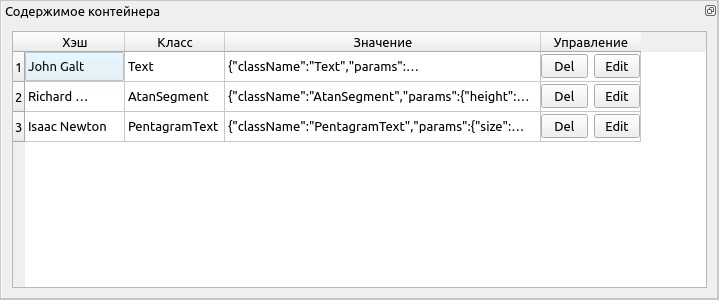
\includegraphics[width=\textwidth]{img/IMG_001.jpg}
    \caption{Отображение контейнера}%
    \label{img:qtable}
\end{figure}

Добавление элемента в контейнер показано на рис.~\ref{img:addfigure}:
\begin{figure}[h]
    \centering
    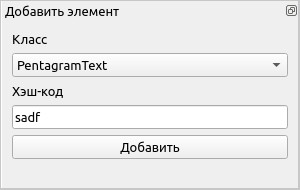
\includegraphics{img/IMG_002.jpg}
    \caption{Добавление элемента в контейнер}%
    \label{img:addfigure}
\end{figure}
\FloatBarrier{}

Настройка параметров добавляемой фигуры представлена на рис.~\ref{img:figparams}:
\begin{figure}[h]
    \centering
    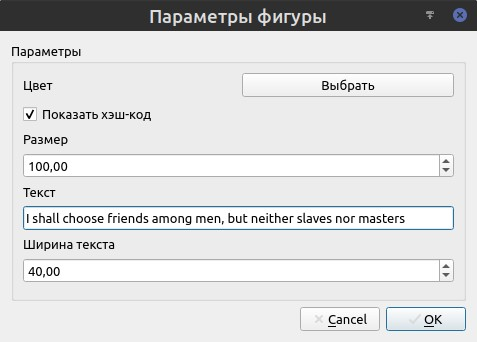
\includegraphics[width=0.7\textwidth]{img/IMG_004.jpg}
    \caption{Настройка параметров фигуры}%
    \label{img:figparams}
\end{figure}

Код диалога, представленного на рис.~\ref{img:figparams} --- в приложениях У, Ф.

\subsection{Отображение графических фигур}
Иерархия графических фигур ЛР1 модифицирована --- класс \texttt{Shape} унаследован от \texttt{QGraphicsItem}, а \texttt{Point} --- от \texttt{QPointF}. Избыточные методы --- уже реализованные в классах Qt --- убраны.

Методы рисования переопределены в наследниках. Коды фигур в приложениях Ж--Р. 

\texttt{QGraphicsItem} настроен, чтобы поддерживать drag\&drop.

Для отображения унаследован класс \texttt{QGraphicsWidget} (код в приложениях С--Т). В нём установлен экземпляр \texttt{QGraphicsScene}, который композирует QGraphicsItem'ы и управляет их отображением.

\texttt{MainWindow} сихронизирует состояние контейнера и сцены, там же находятся фабрики фигур.

Пример отображения фигур представлен на~\ref{img:figures}.

\begin{figure}[h]
    \centering
    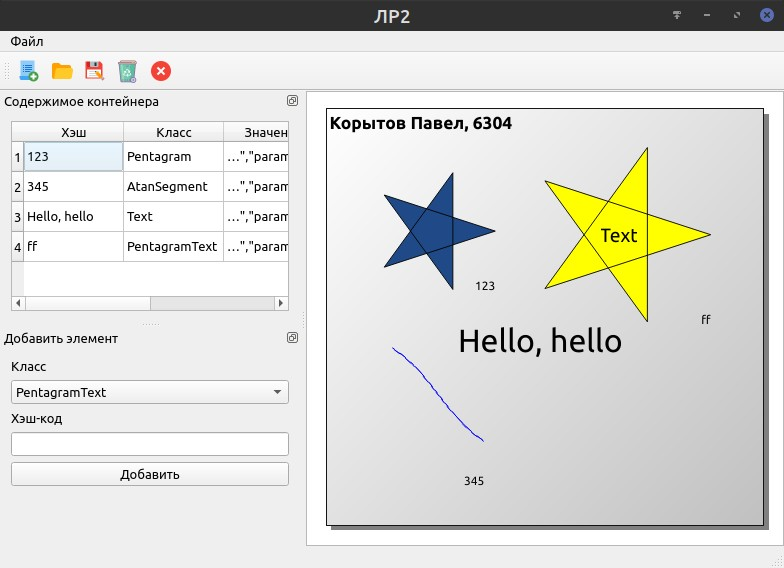
\includegraphics[width=\textwidth]{img/IMG_005.jpg}
    \caption{Отображение фигур}%
    \label{img:figures}
\end{figure}

\subsection{Сериализация}
Для сериализации и десериализации выбран формат JSON в реализации \texttt{QJson}.

У фигур определен метод \texttt{toJSON}, конвертирующий их в JSON-объекты. При сохранении в ходе итерации по контейнеру вызывается этот метод, общий результат сохраняется в JSON-файл. Пример такого файлы представлен в приложении Ч.

При десериализации содержимое контейнера и сцены восстанавливается по файлу.

\section{Выводы}
Произведено создание графического приложения с использованием фреймворка Qt. Изучена реализация паттерна MVC в Qt, использование компонентов отображения и работы с файлами.

\printbibliography{}
\addcontentsline{toc}{section}{Список литературы}

\phantomsection{}\addcontentsline{toc}{section}{Приложения}
\Addon{Приложение А}{Исходный код main.cpp}{../src/main.cpp}
\Addon{Приложение Б}{Исходный код mainwindow.h}{../src/mainwindow.h}
\Addon{Приложение В}{Исходный код mainwindow.cpp}{../src/mainwindow.cpp}
\Addon{Приложение Г}{Исходный код hashMap.h}{../src/hashMap.h}
\Addon{Приложение Е}{Исходный код exception.h}{../src/exception.h}
\Addon{Приложение Ж}{Исходный код figures/shape.h}{../src/figures/shape.h}
\Addon{Приложение З}{Исходный код figures/shape.cpp}{../src/figures/shape.cpp}
\Addon{Приложение И}{Исходный код figures/atansegment.h}{../src/figures/atansegment.h}
\Addon{Приложение К}{Исходный код figures/atansegment.cpp}{../src/figures/atansegment.cpp}
\Addon{Приложение Л}{Исходный код figures/pentagram.h}{../src/figures/pentagram.h}
\Addon{Приложение М}{Исходный код figures/pentagram.cpp}{../src/figures/pentagram.cpp}
\Addon{Приложение Н}{Исходный код figures/text.h}{../src/figures/text.h}
\Addon{Приложение О}{Исходный код figures/text.cpp}{../src/figures/text.cpp}
\Addon{Приложение П}{Исходный код figures/pentagramtext.h}{../src/figures/pentagramtext.h}
\Addon{Приложение Р}{Исходный код figures/pentagramtext.cpp}{../src/figures/pentagramtext.cpp}
\Addon{Приложение С}{Исходный код graphwidget.h}{../src/graphwidget.h}
\Addon{Приложение Т}{Исходный код graphwidget.cpp}{../src/graphwidget.cpp}
\Addon{Приложение У}{Исходный код adddialog.h}{../src/adddialog.h}
\Addon{Приложение Ф}{Исходный код adddialog.cpp}{../src/adddialog.cpp}
\Addon{Приложение Х}{Исходный код point.h}{../src/point.h}
\Addon{Приложение Ц}{Исходный код point.cpp}{../src/point.cpp}
\Addon{Приложение Ч}{Пример сериалиазации}{./example.json}

\end{document}
